% Compile with: pdflatex -interaction=nonstopmode -halt-on-error docs/secure_email_presentation.tex
\documentclass[aspectratio=169]{beamer}

\usepackage{graphicx}

\usetheme{Madrid}
\usecolortheme{default}
\setbeamertemplate{navigation symbols}{}
\graphicspath{{docs/test_frontend_screenshots/}{test_frontend_screenshots/}}

\title{Smart Secure Email System}
\subtitle{Assignment-Aligned Project Presentation With Live Frontend Evidence}
\author{Secure Email Project}
\date{April 13, 2026}

\begin{document}

\begin{frame}
  \titlepage
\end{frame}

\begin{frame}{Assignment Objective}
  \begin{itemize}
    \item Build a \textbf{usable}, \textbf{testable}, and \textbf{security-aware} email system in a local environment.
    \item Implement both \textbf{server} and \textbf{client} components.
    \item Add at least basic \textbf{intelligent features}.
    \item Provide \textbf{reproducible test steps and results}.
    \item Avoid using a mature open-source email system as the core implementation.
  \end{itemize}
\end{frame}

\begin{frame}{Design Strategy}
  \begin{itemize}
    \item Use a custom HTTPS/JSON mail protocol instead of SMTP/IMAP as the core runtime.
    \item Simulate \textbf{two isolated email domains} with two independent FastAPI servers.
    \item Keep request handling short and safe, then move slow work to a \textbf{queue-backed worker model}.
    \item Treat security as part of system design, not an afterthought:
    \begin{itemize}
      \item authentication
      \item replay protection
      \item rate limiting
      \item relay verification
      \item attachment safety
    \end{itemize}
  \end{itemize}
\end{frame}

\begin{frame}{Architecture Overview}
  \begin{columns}[T]
    \column{0.48\textwidth}
    \textbf{Client Side}
    \begin{itemize}
      \item Browser frontend
      \item CLI client
      \item Signed authenticated requests
    \end{itemize}

    \textbf{Server Side}
    \begin{itemize}
      \item Domain A server
      \item Domain B server
      \item Auth, mailbox, attachments, relay
    \end{itemize}

    \column{0.48\textwidth}
    \textbf{Workers}
    \begin{itemize}
      \item Local delivery jobs
      \item Remote relay jobs
      \item Inbound insertion jobs
    \end{itemize}

    \textbf{Storage}
    \begin{itemize}
      \item SQLite per domain
      \item Attachment blob store
      \item Audit log
    \end{itemize}
  \end{columns}
\end{frame}

\begin{frame}{Server Management Requirement}
  \begin{itemize}
    \item Two servers run at the same time:
    \begin{itemize}
      \item \texttt{a.test} on port 8443
      \item \texttt{b.test} on port 9443
    \end{itemize}
    \item The two systems can send mail to each other through authenticated relay endpoints.
    \item Their storage is logically isolated:
    \begin{itemize}
      \item separate database files
      \item separate attachment roots
      \item separate security logs
    \end{itemize}
    \item One server never directly reads or writes the other domain's user data directory.
  \end{itemize}
\end{frame}

\begin{frame}{Client Management Requirement}
  \begin{itemize}
    \item Registration and login
    \item Compose mail, inbox, sent, drafts, search, and calendar / follow-up views
    \item Saved groups integrated directly into the main compose form
    \item Quick reply support with subject/thread context and manual compose staging
    \item Attachment upload, saved-attachment management, preview, compression, and reuse
    \item Mail recall for sent messages
    \item Quick actions designed from the user perspective:
    \begin{itemize}
      \item add TODO
      \item add calendar event
      \item acknowledge message
      \item report suspicious mail
    \end{itemize}
  \end{itemize}
\end{frame}

\begin{frame}{Intelligent Features Implemented}
  \begin{itemize}
    \item \textbf{Keyword extraction}
    \item \textbf{Mail classification}
    \item \textbf{Fuzzy search} for messages and contacts
    \item \textbf{Quick reply suggestions} and AI-assisted drafting
    \item \textbf{Phishing / suspicious-mail heuristics}
    \item \textbf{Attachment deduplication} as a storage-aware optimization
    \item \textbf{Local smart module integration} through Ollama when available, with safe fallback
  \end{itemize}

  \vspace{0.4em}
  This exceeds the ``at least 2 algorithm-enhanced features'' requirement.
\end{frame}

\begin{frame}{Security and Stability Design}
  \begin{itemize}
    \item Passwords are stored with \textbf{Argon2id}, never in plaintext.
    \item Sensitive database fields and stored secrets are encrypted at rest.
    \item Post-login requests use:
    \begin{itemize}
      \item session token
      \item request ID
      \item nonce
      \item timestamp
      \item sequence number
      \item HMAC over canonical request content
    \end{itemize}
    \item Login anti-brute-force protection:
    \begin{itemize}
      \item short-term lockout
      \item rate limiting
    \end{itemize}
    \item Send/upload abuse control with rate limits
    \item Relay authentication between the two domains
    \item ECC-based end-to-end encryption for text messages
    \item Local-only smart-module policy to reduce data leakage risk
    \item Recall verification to prevent incorrect recall execution
  \end{itemize}
\end{frame}

\begin{frame}{How Secure Post-Login Interaction Works}
  \begin{enumerate}
    \item User logs in once and gets a session token plus session key.
    \item Sensitive requests include request metadata headers.
    \item Client computes an HMAC over method, path, metadata, and body.
    \item Server verifies:
    \begin{itemize}
      \item session validity
      \item timestamp window
      \item nonce uniqueness
      \item sequence progression
      \item HMAC correctness
    \end{itemize}
    \item Replayed or tampered requests are rejected.
  \end{enumerate}
\end{frame}

\begin{frame}{Queue and Concurrency Model}
  \begin{itemize}
    \item Request handlers do not wait for all relay work inline.
    \item A send request:
    \begin{itemize}
      \item validates authentication and policy
      \item writes sender-side state
      \item inserts delivery jobs into a persistent SQLite queue
      \item returns quickly with \texttt{queued}
    \end{itemize}
    \item Worker threads handle:
    \begin{itemize}
      \item local delivery
      \item remote relay
      \item inbound inbox insertion
    \end{itemize}
    \item This improves stability under concurrent client activity.
  \end{itemize}
\end{frame}

\begin{frame}{Attachment and Storage Safety}
  \begin{itemize}
    \item All attachment file types are accepted for normal mail workflows.
    \item Validation uses magic bytes, not only file extension.
    \item Image AI review and image transforms run only for image attachments.
    \item Files are stored with generated blob paths, not user-controlled paths.
    \item Blob storage uses SHA-256-based deduplication.
    \item Compressed copies can replace draft-linked originals without breaking immutable mail history.
    \item Attachment access is protected by mailbox ownership checks.
  \end{itemize}
\end{frame}

\begin{frame}{Live Frontend Overview}
  \begin{center}
    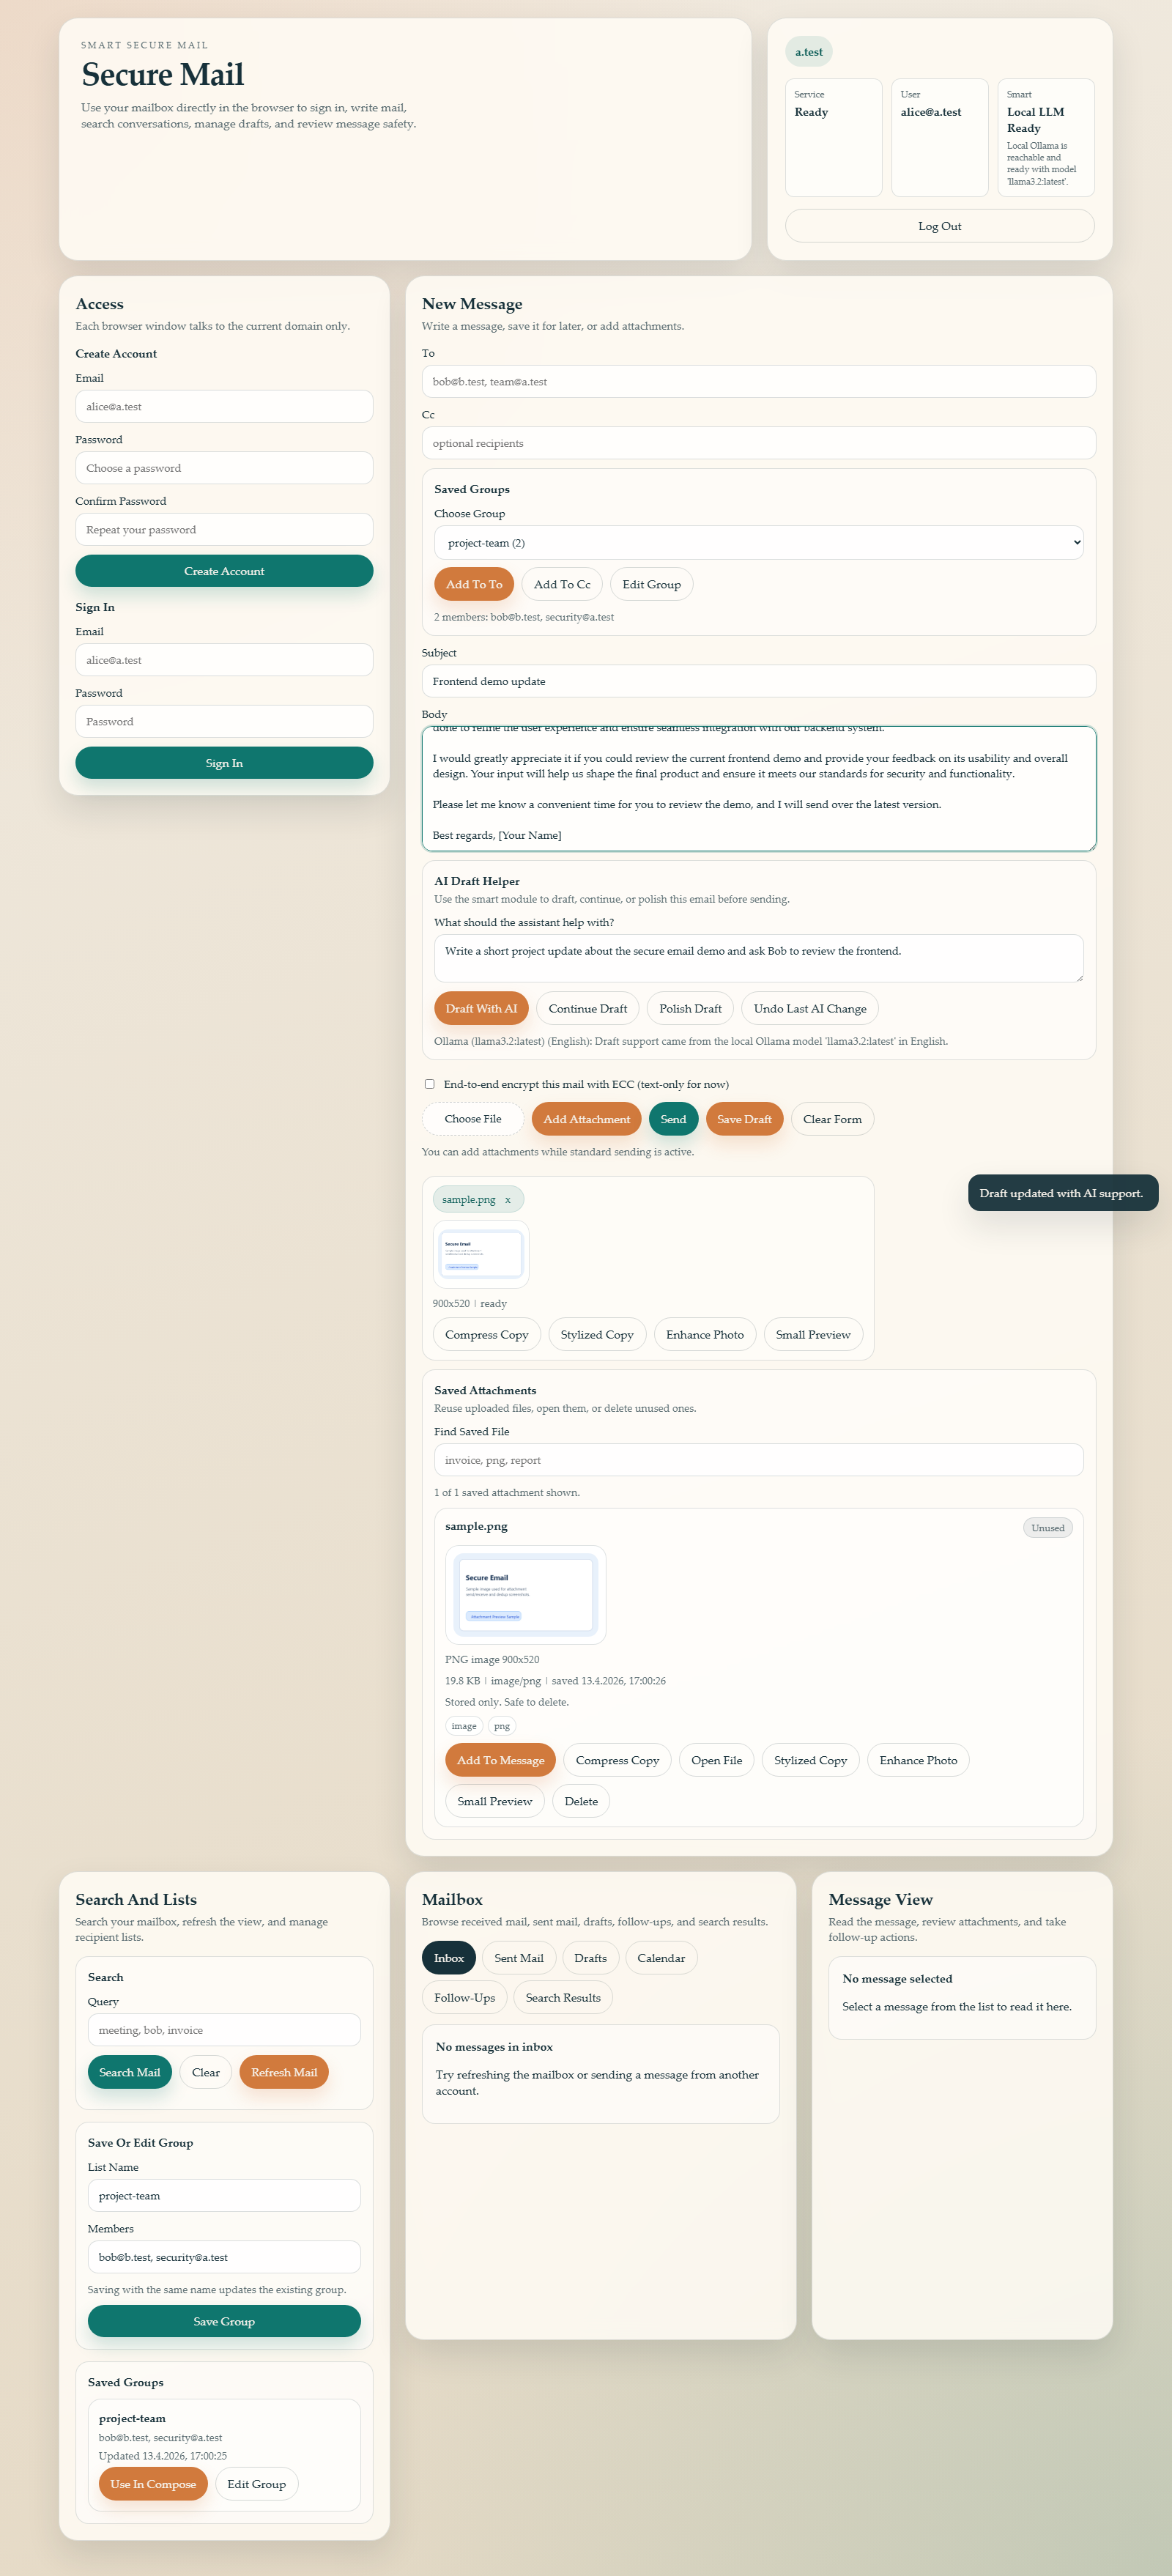
\includegraphics[height=0.72\textheight,keepaspectratio]{01_main_console_real.png}
  \end{center}
  \vspace{0.4em}
  \small The browser frontend now combines login, AI drafting, saved groups, saved attachments, and the main compose workflow in one place.
\end{frame}

\begin{frame}{Delivery And Attachment Evidence}
  \begin{columns}[T]
    \column{0.49\textwidth}
    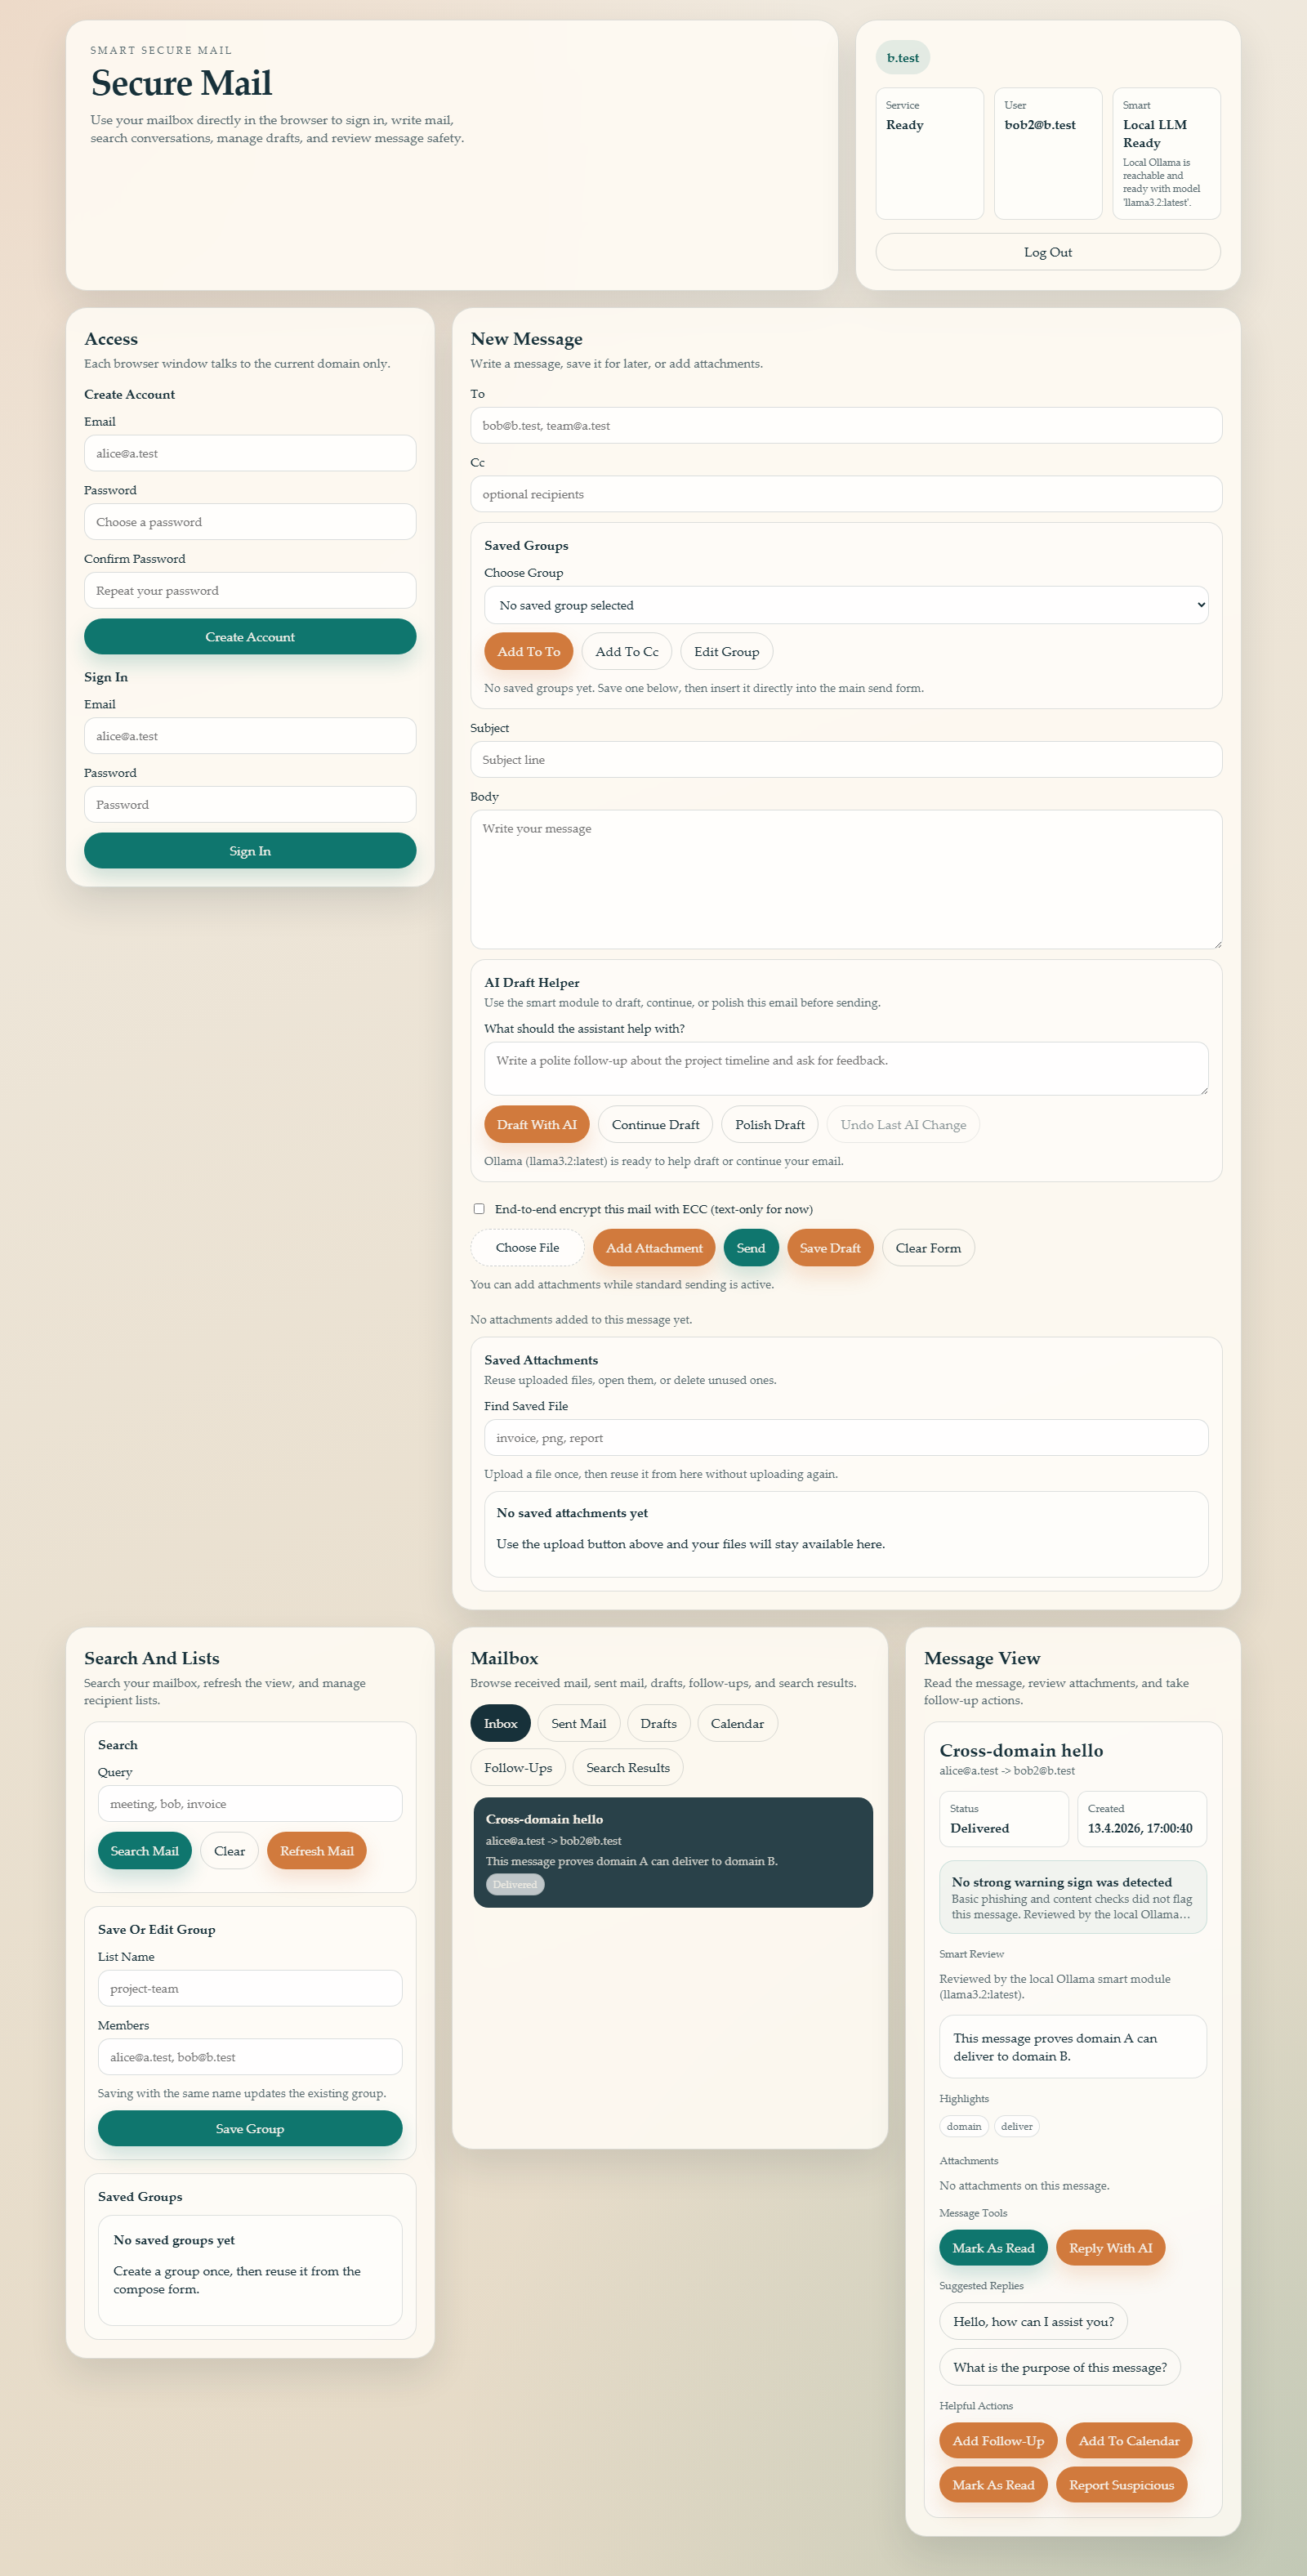
\includegraphics[width=\textwidth,height=0.50\textheight,keepaspectratio]{02_cross_domain_delivery_real.png}

    \vspace{0.3em}
    \scriptsize Cross-domain delivery from \texttt{a.test} to \texttt{b.test}.

    \column{0.49\textwidth}
    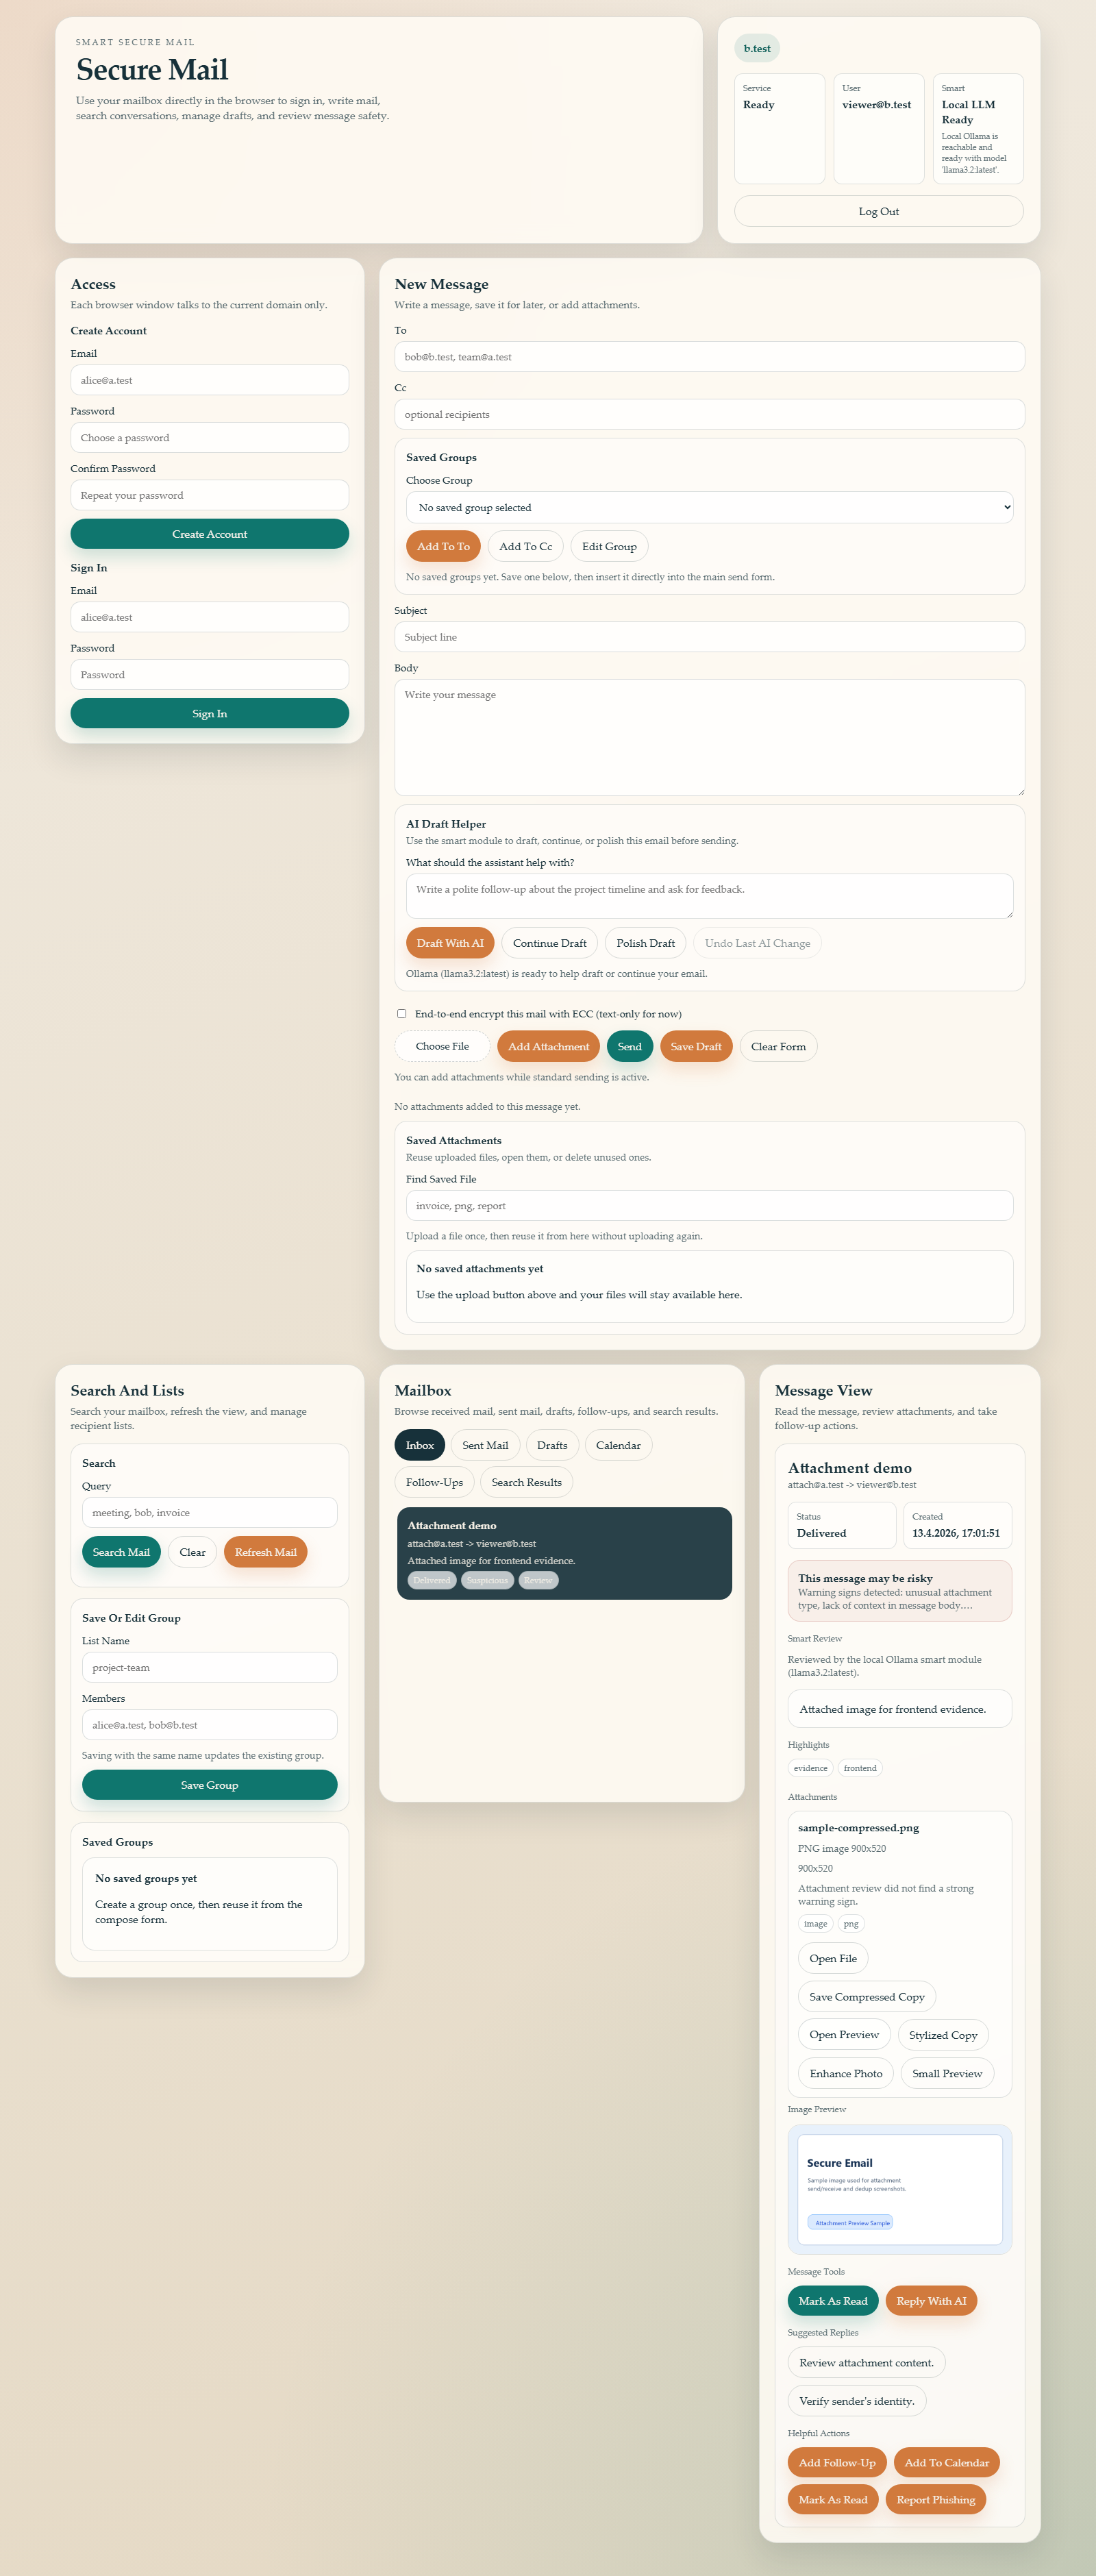
\includegraphics[width=\textwidth,height=0.50\textheight,keepaspectratio]{08_attachment_send_receive_real.png}

    \vspace{0.3em}
    \scriptsize Receiver-side attachment preview opened from the real inbox.
  \end{columns}
\end{frame}

\begin{frame}{Security Lab: Threat Cases}
  \begin{columns}[T]
    \column{0.56\textwidth}
    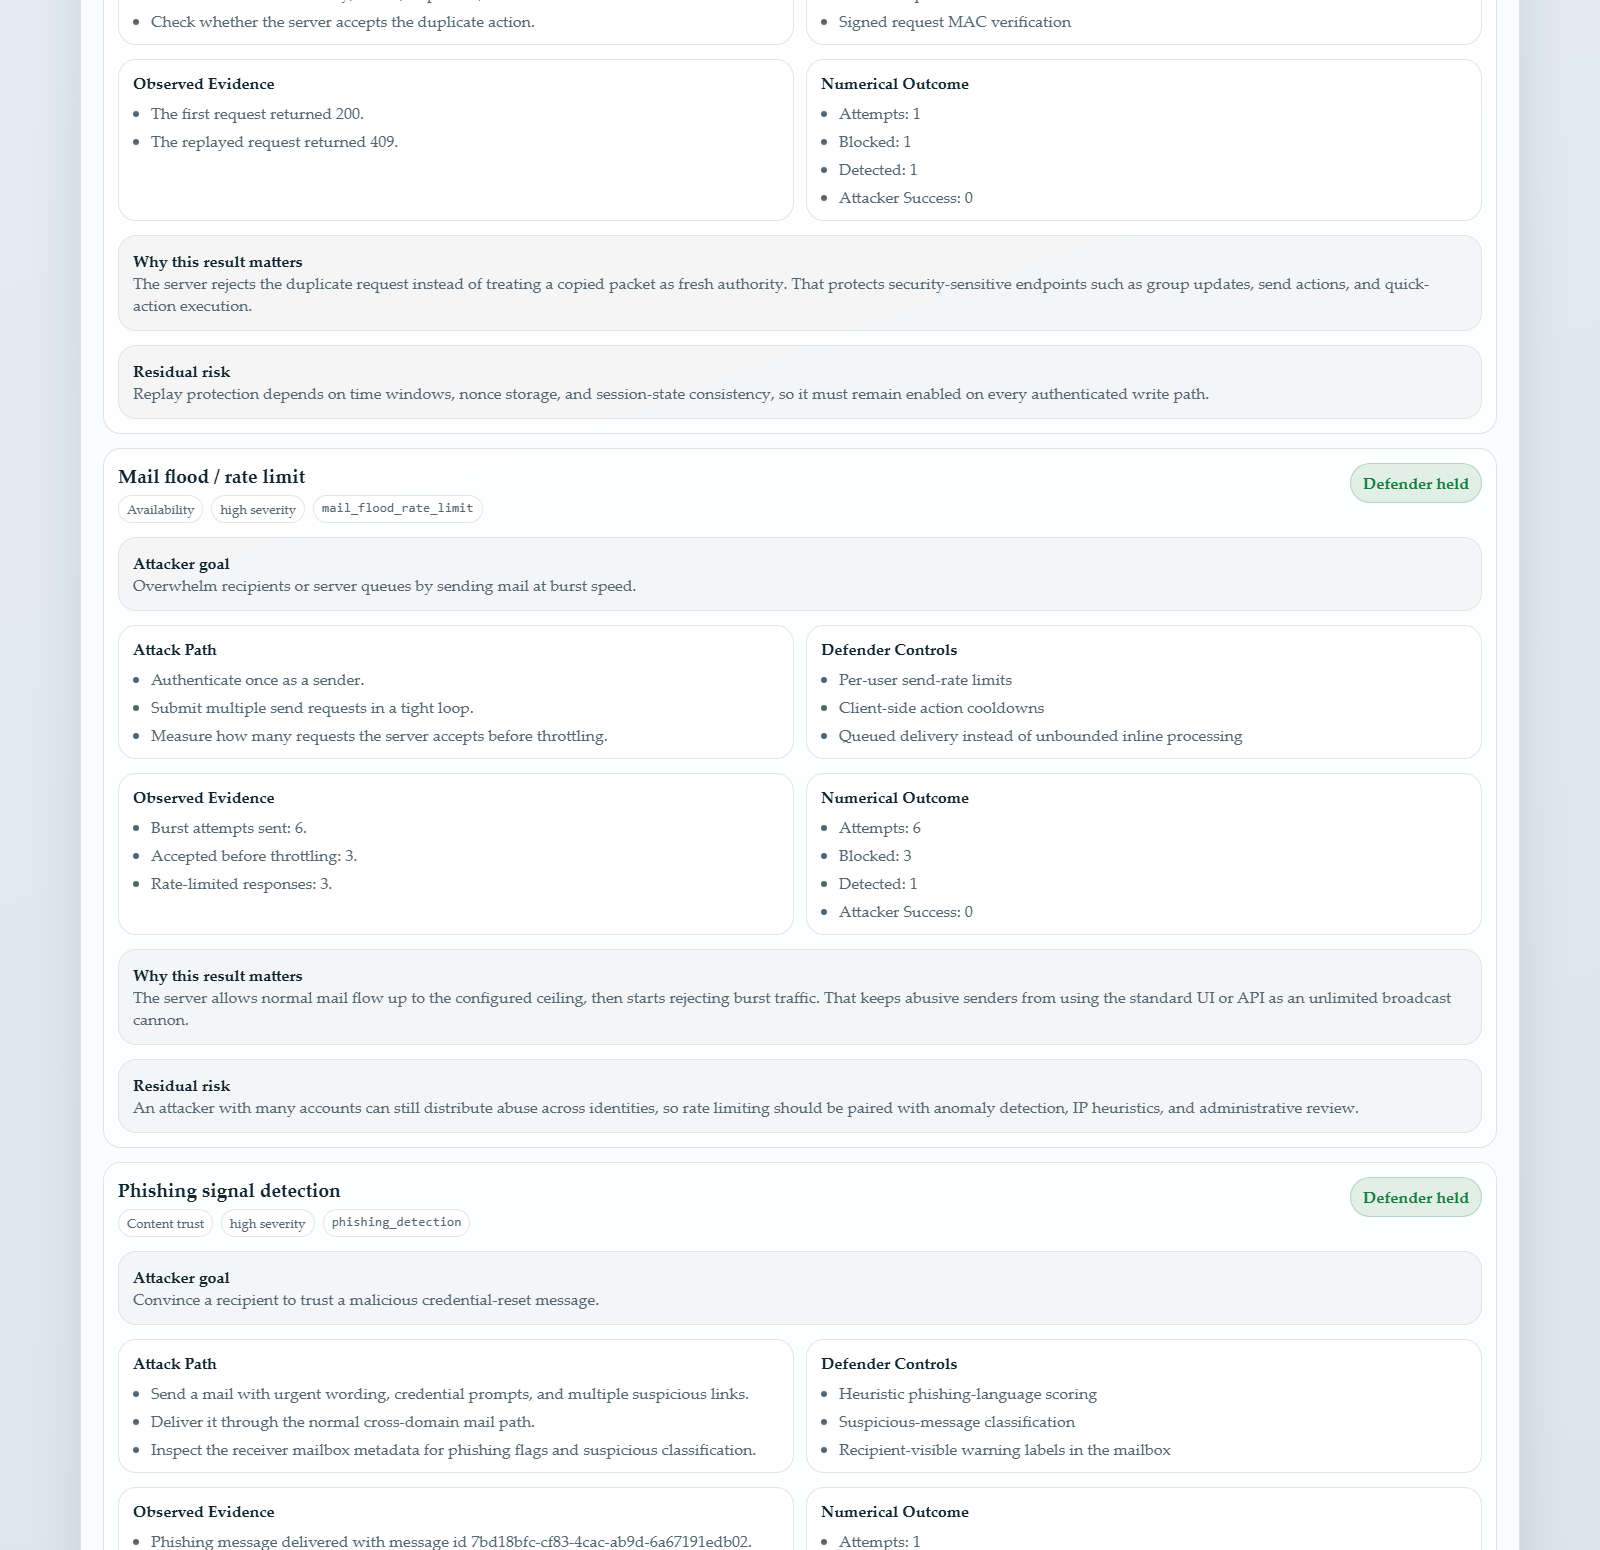
\includegraphics[width=\textwidth,height=0.66\textheight,keepaspectratio]{09_security_lab_scenarios_top_crop.png}

    \vspace{0.2em}
    \scriptsize Zoomed evidence from the live security-lab scenario area.

    \column{0.42\textwidth}
    \scriptsize
    \begin{itemize}
      \item \textbf{Brute-force login}: attacker repeatedly guesses one mailbox password.
      \item \textbf{Replay attack}: attacker resends one previously valid signed request.
      \item \textbf{Mail flood}: attacker sends bursts to overload recipients or queues.
      \item \textbf{Phishing detection}: attacker sends urgent credential-reset style mail.
      \item \textbf{Malicious attachment}: attacker disguises unsafe bytes as an image.
    \end{itemize}
    \vspace{0.4em}
    \scriptsize The lab executes these drills through the real endpoints, so the cases match the actual threat surface of the email system.
  \end{columns}
\end{frame}

\begin{frame}{Security Lab: System Reactions}
  \begin{columns}[T]
    \column{0.56\textwidth}
    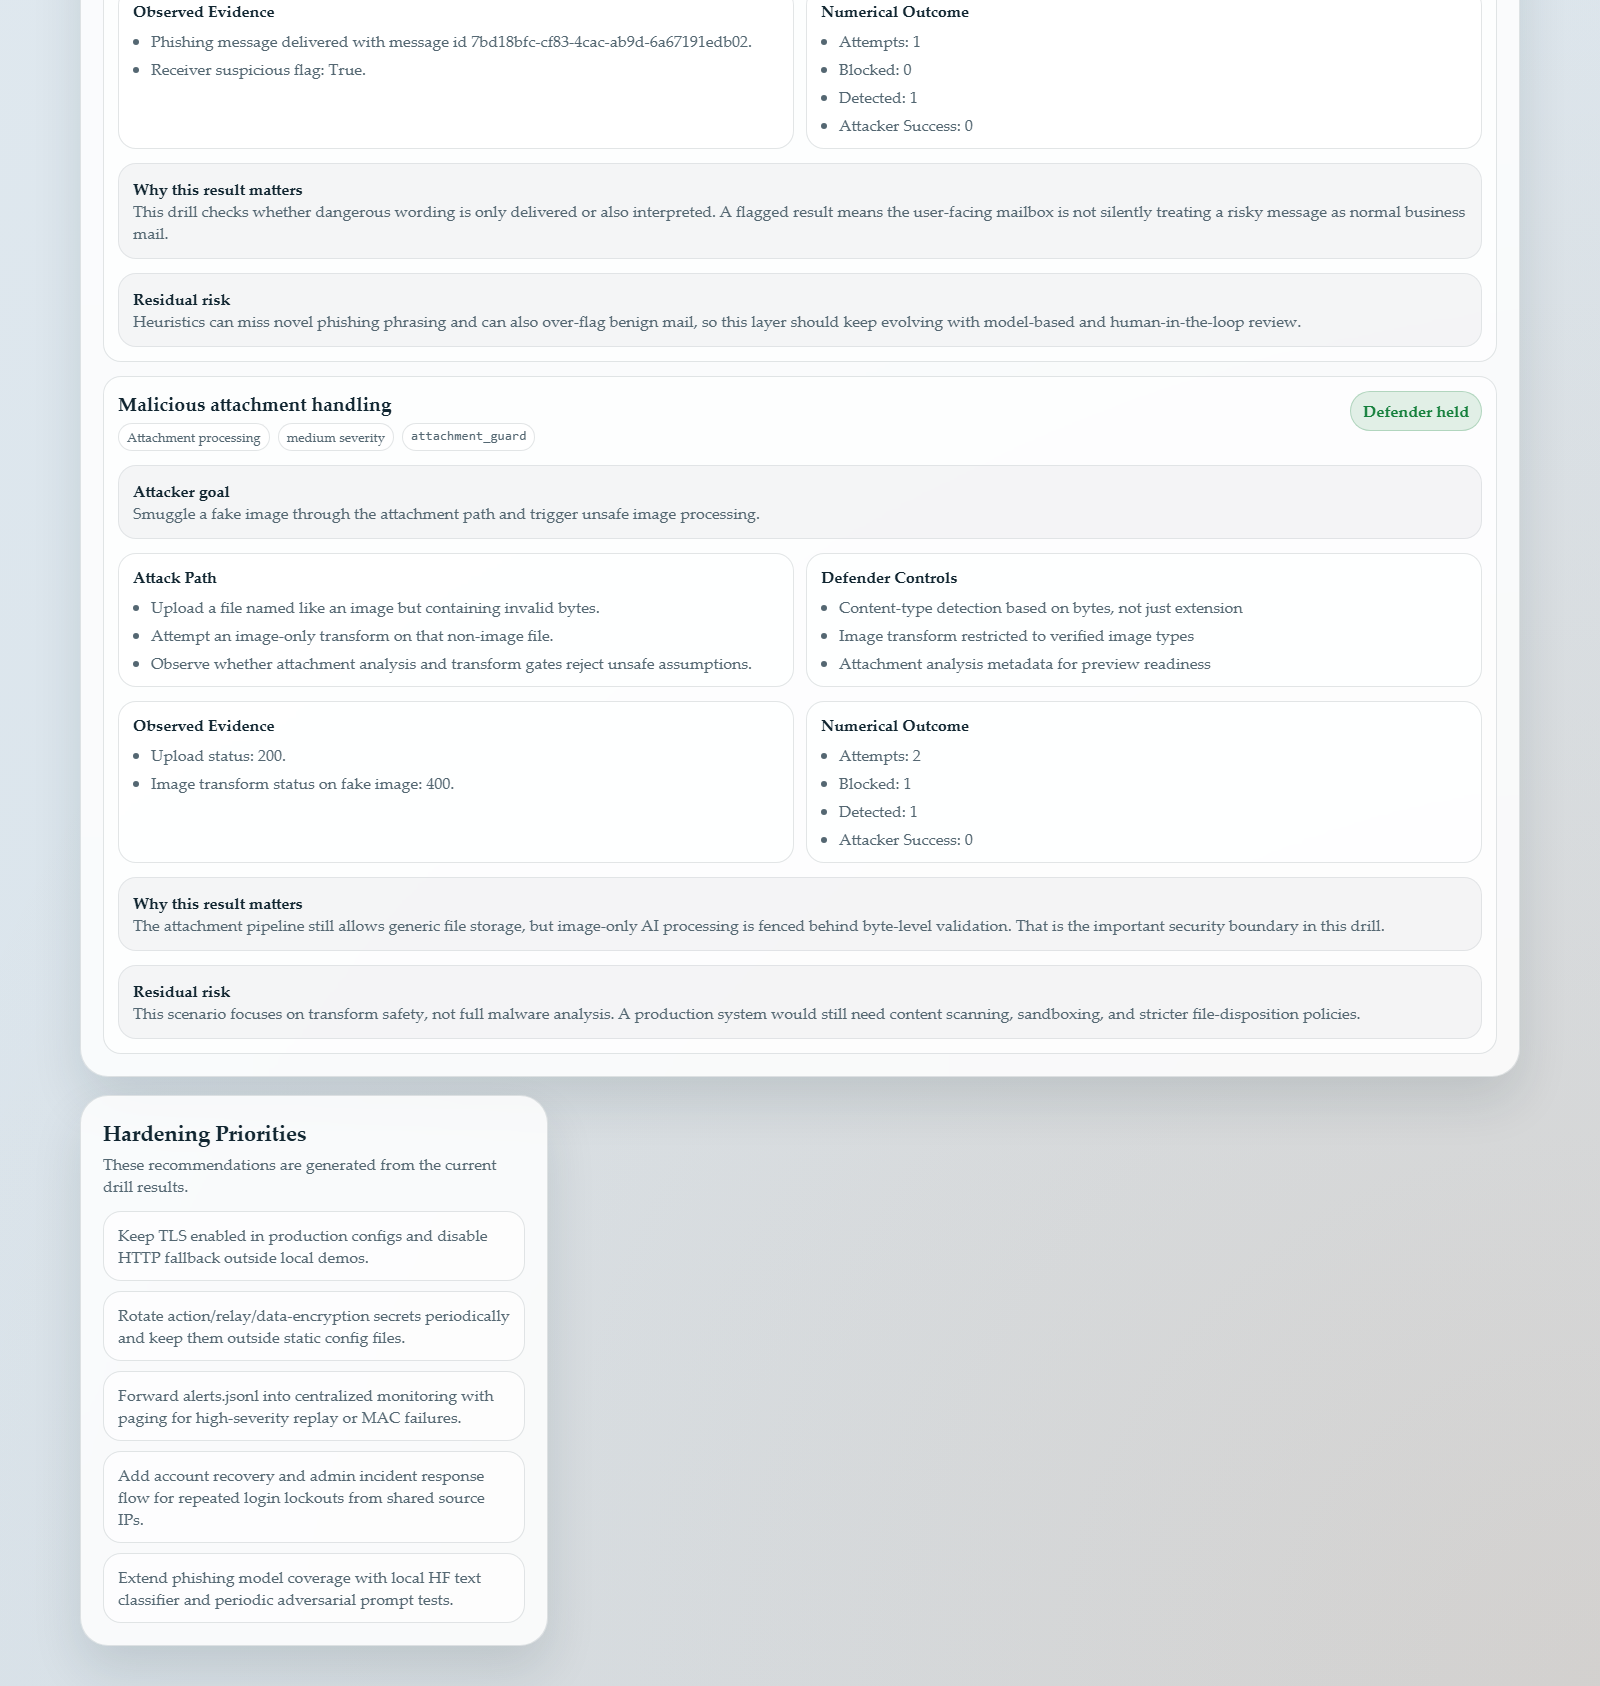
\includegraphics[width=\textwidth,height=0.66\textheight,keepaspectratio]{09_security_lab_scenarios_bottom_crop.png}

    \vspace{0.2em}
    \scriptsize Second zoomed section of the same lab page, showing more scenario evidence and follow-up recommendations.

    \column{0.42\textwidth}
    \scriptsize
    \begin{itemize}
      \item Brute-force login: the account is temporarily locked and the attacker is slowed by \texttt{Retry-After}.
      \item Replay attack: copied requests are rejected by nonce tracking, sequence checks, and MAC verification.
      \item Mail flood: burst sending is throttled after the safe configured limit.
      \item Phishing mail: the inbox labels risky content as suspicious instead of showing it as normal mail.
      \item Malicious attachment: fake image bytes cannot enter the image-only analysis and transform path.
    \end{itemize}
    \vspace{0.3em}
    \scriptsize Each scenario card also records attacker goal, attack path, defender controls, observed evidence, and residual risk.
  \end{columns}
\end{frame}

\begin{frame}{Abuse Protection Evidence}
  \begin{columns}[T]
    \column{0.49\textwidth}
    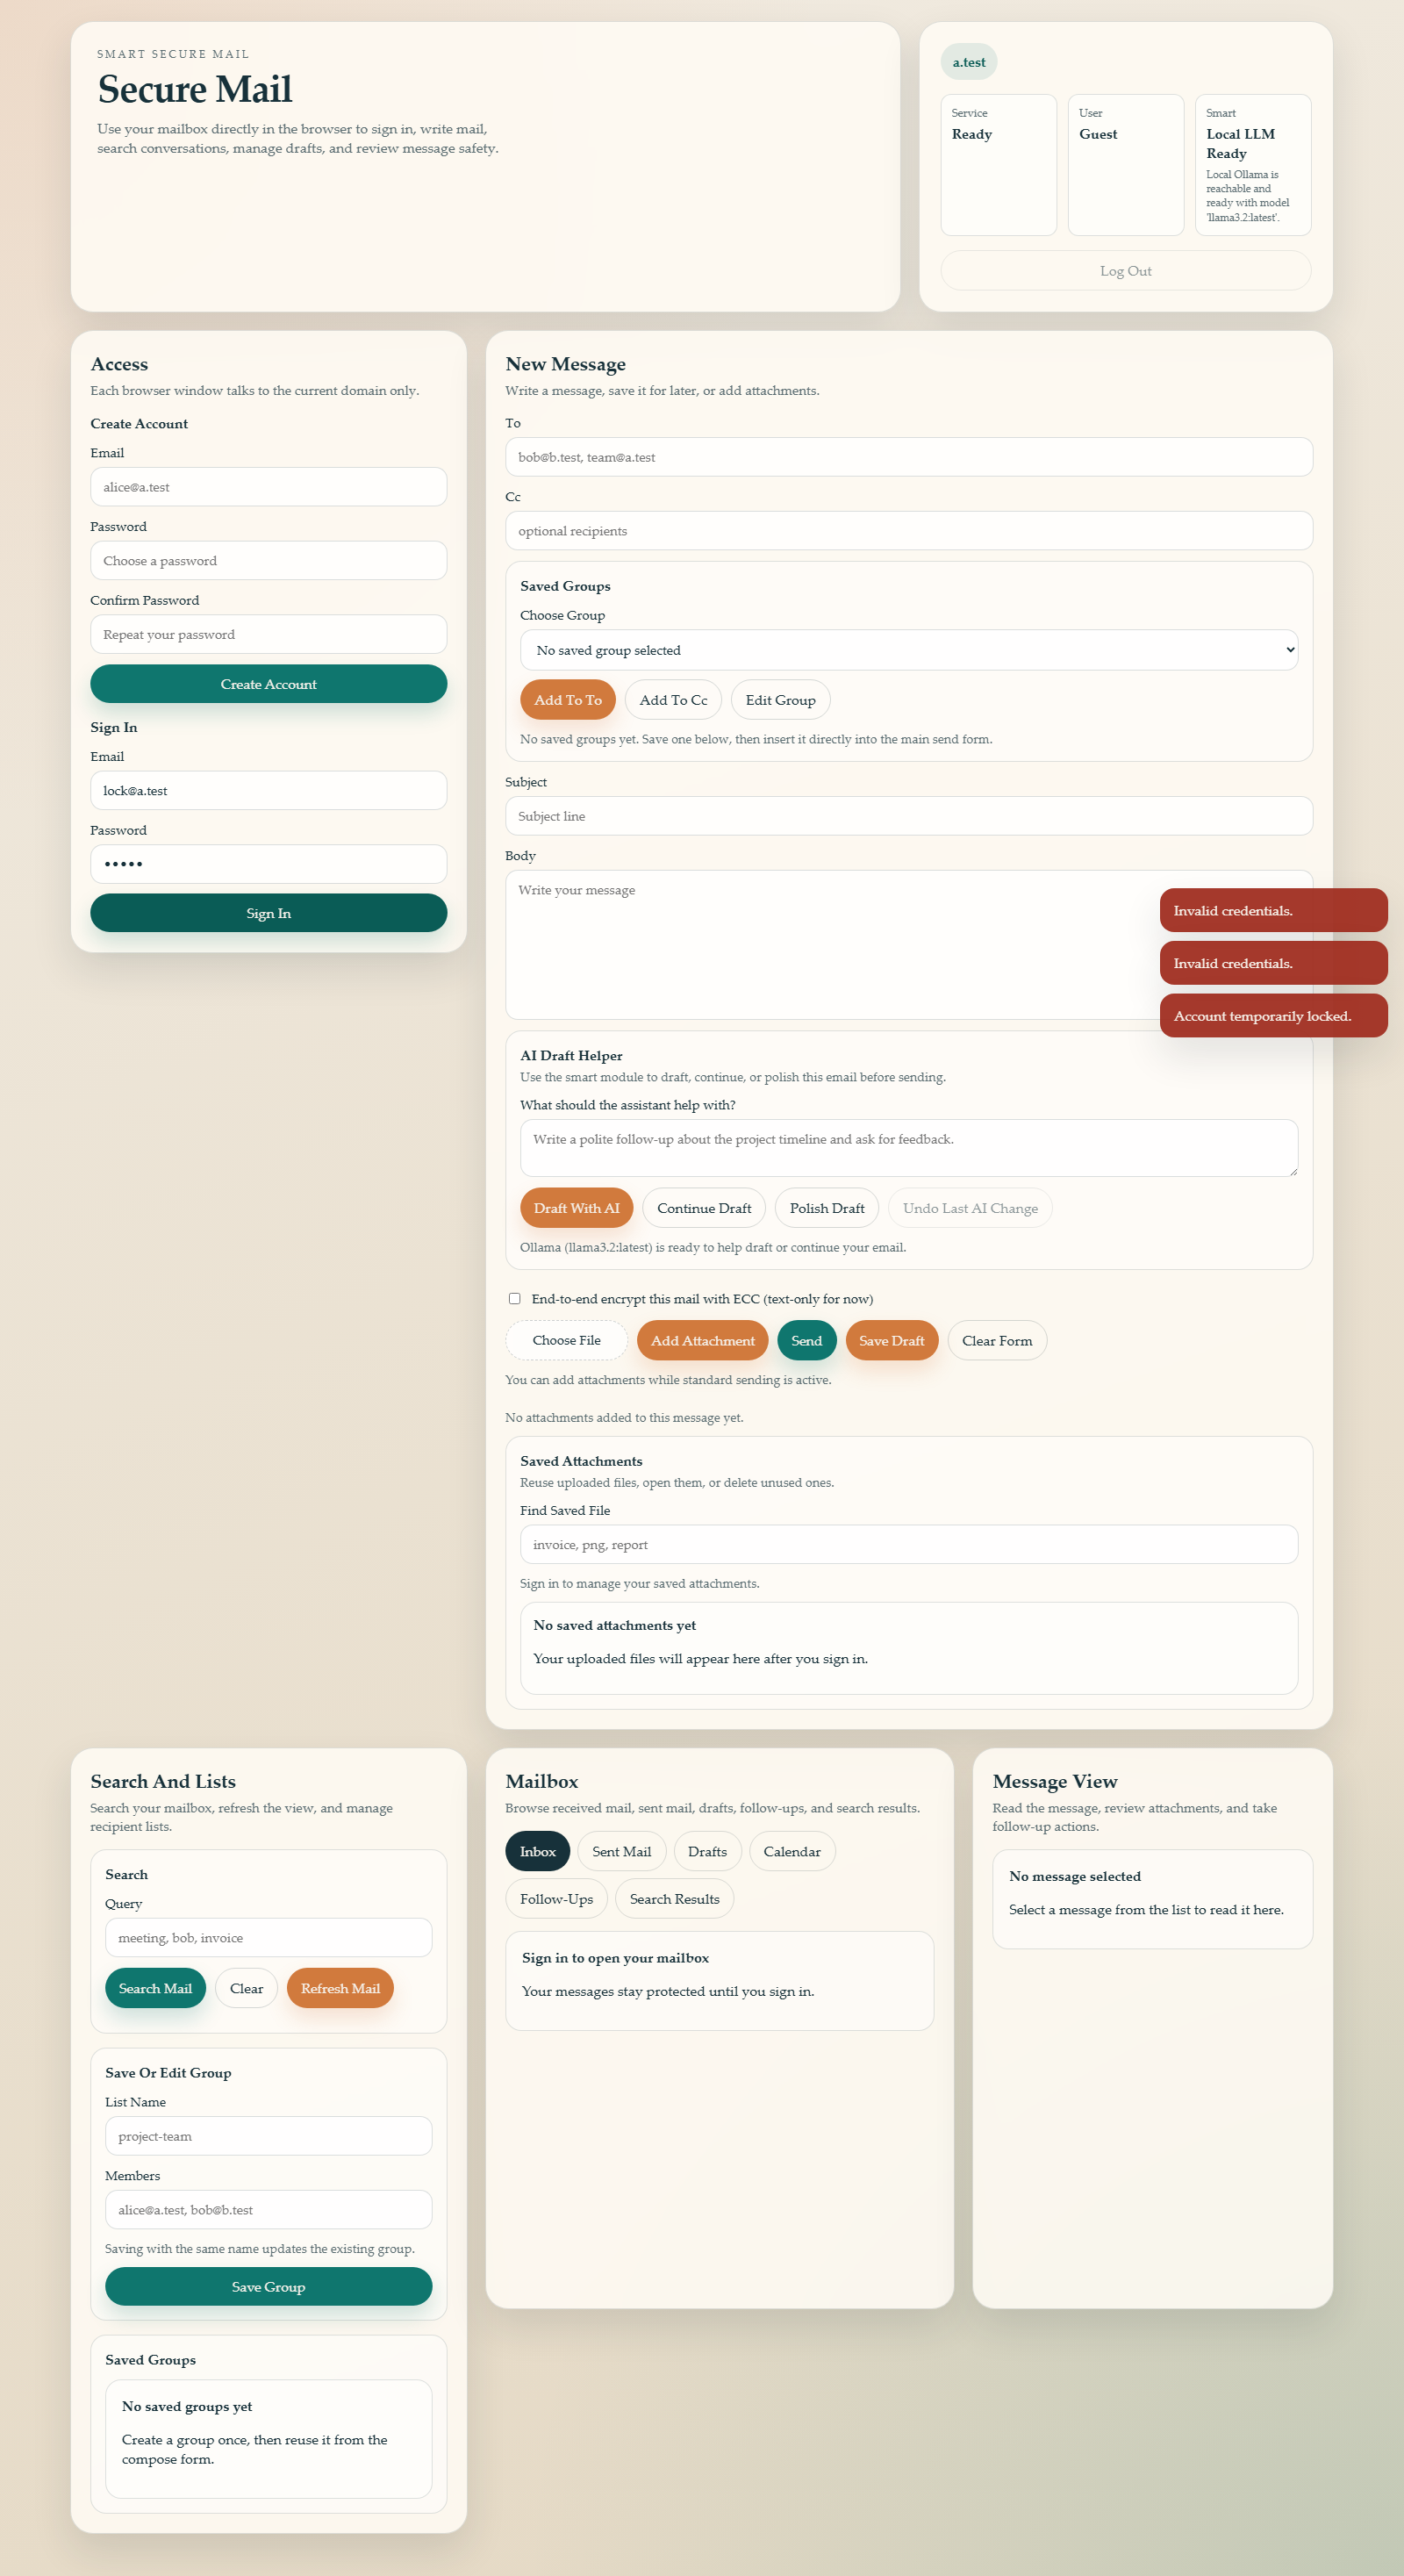
\includegraphics[width=\textwidth,height=0.50\textheight,keepaspectratio]{04_bruteforce_lockout_real.png}

    \vspace{0.3em}
    \scriptsize Brute-force login protection with temporary lockout.

    \column{0.49\textwidth}
    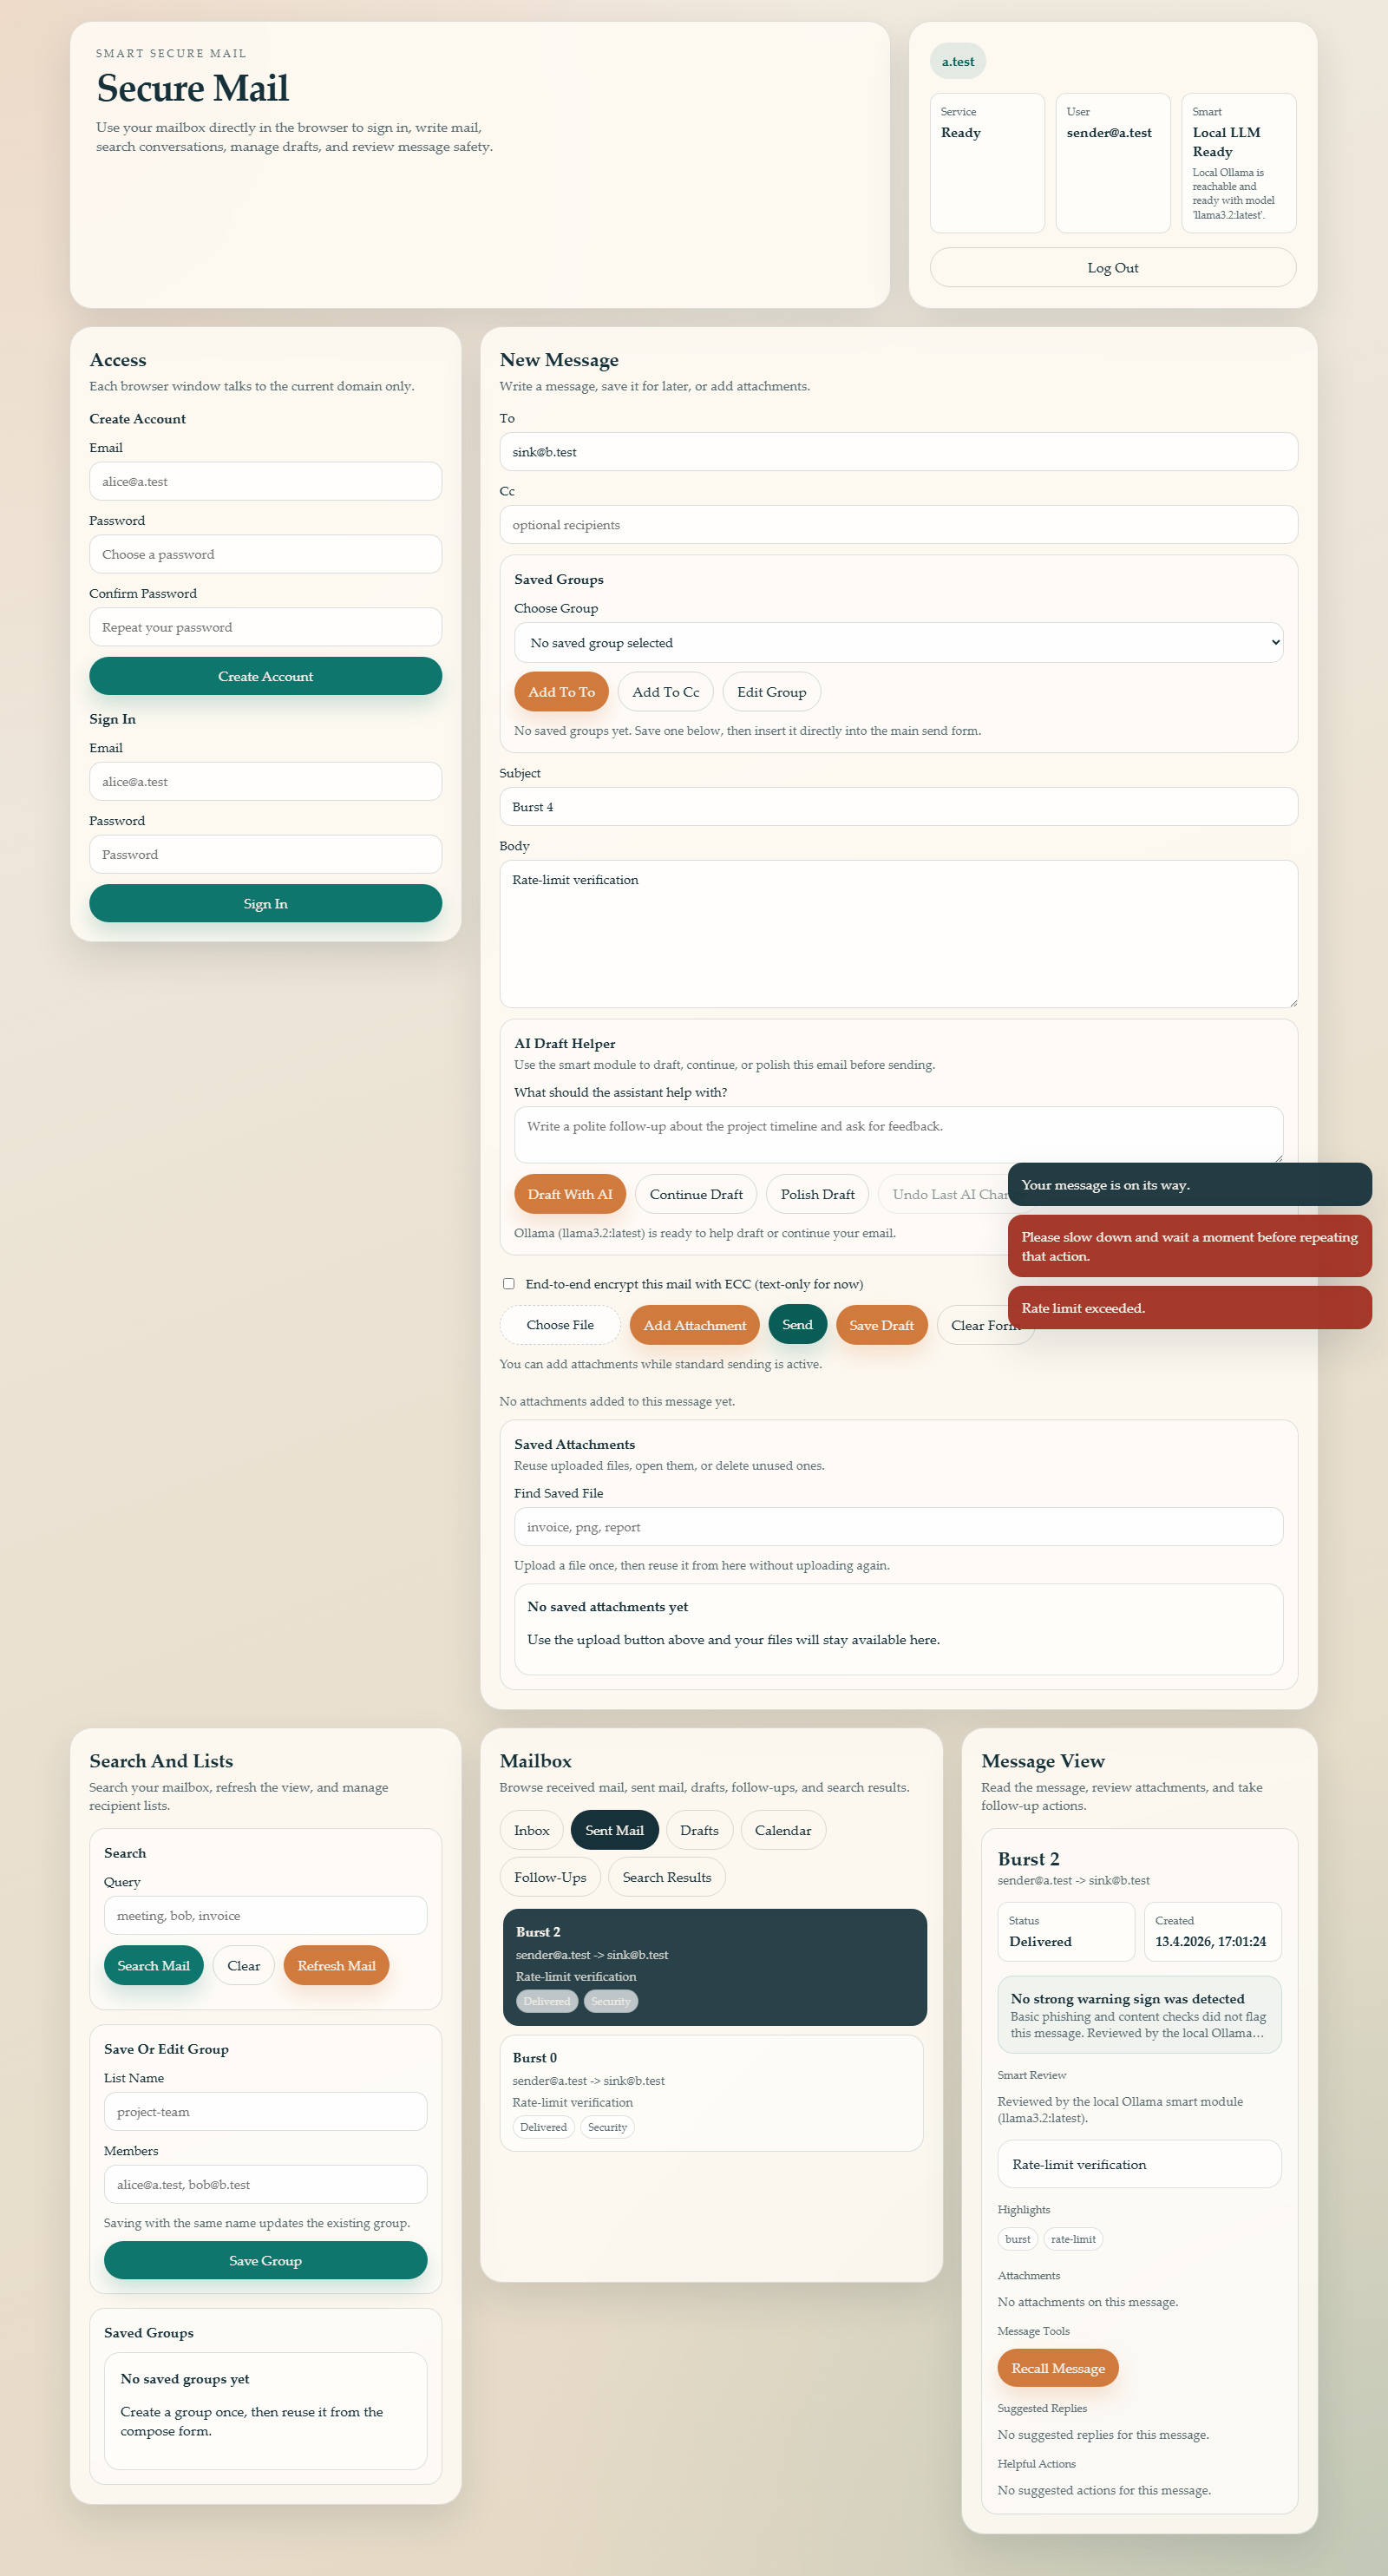
\includegraphics[width=\textwidth,height=0.50\textheight,keepaspectratio]{05_send_rate_limit_real.png}

    \vspace{0.3em}
    \scriptsize High-frequency send attempts blocked in the frontend.
  \end{columns}
\end{frame}

\begin{frame}{Concurrency And Storage Evidence}
  \begin{columns}[T]
    \column{0.49\textwidth}
    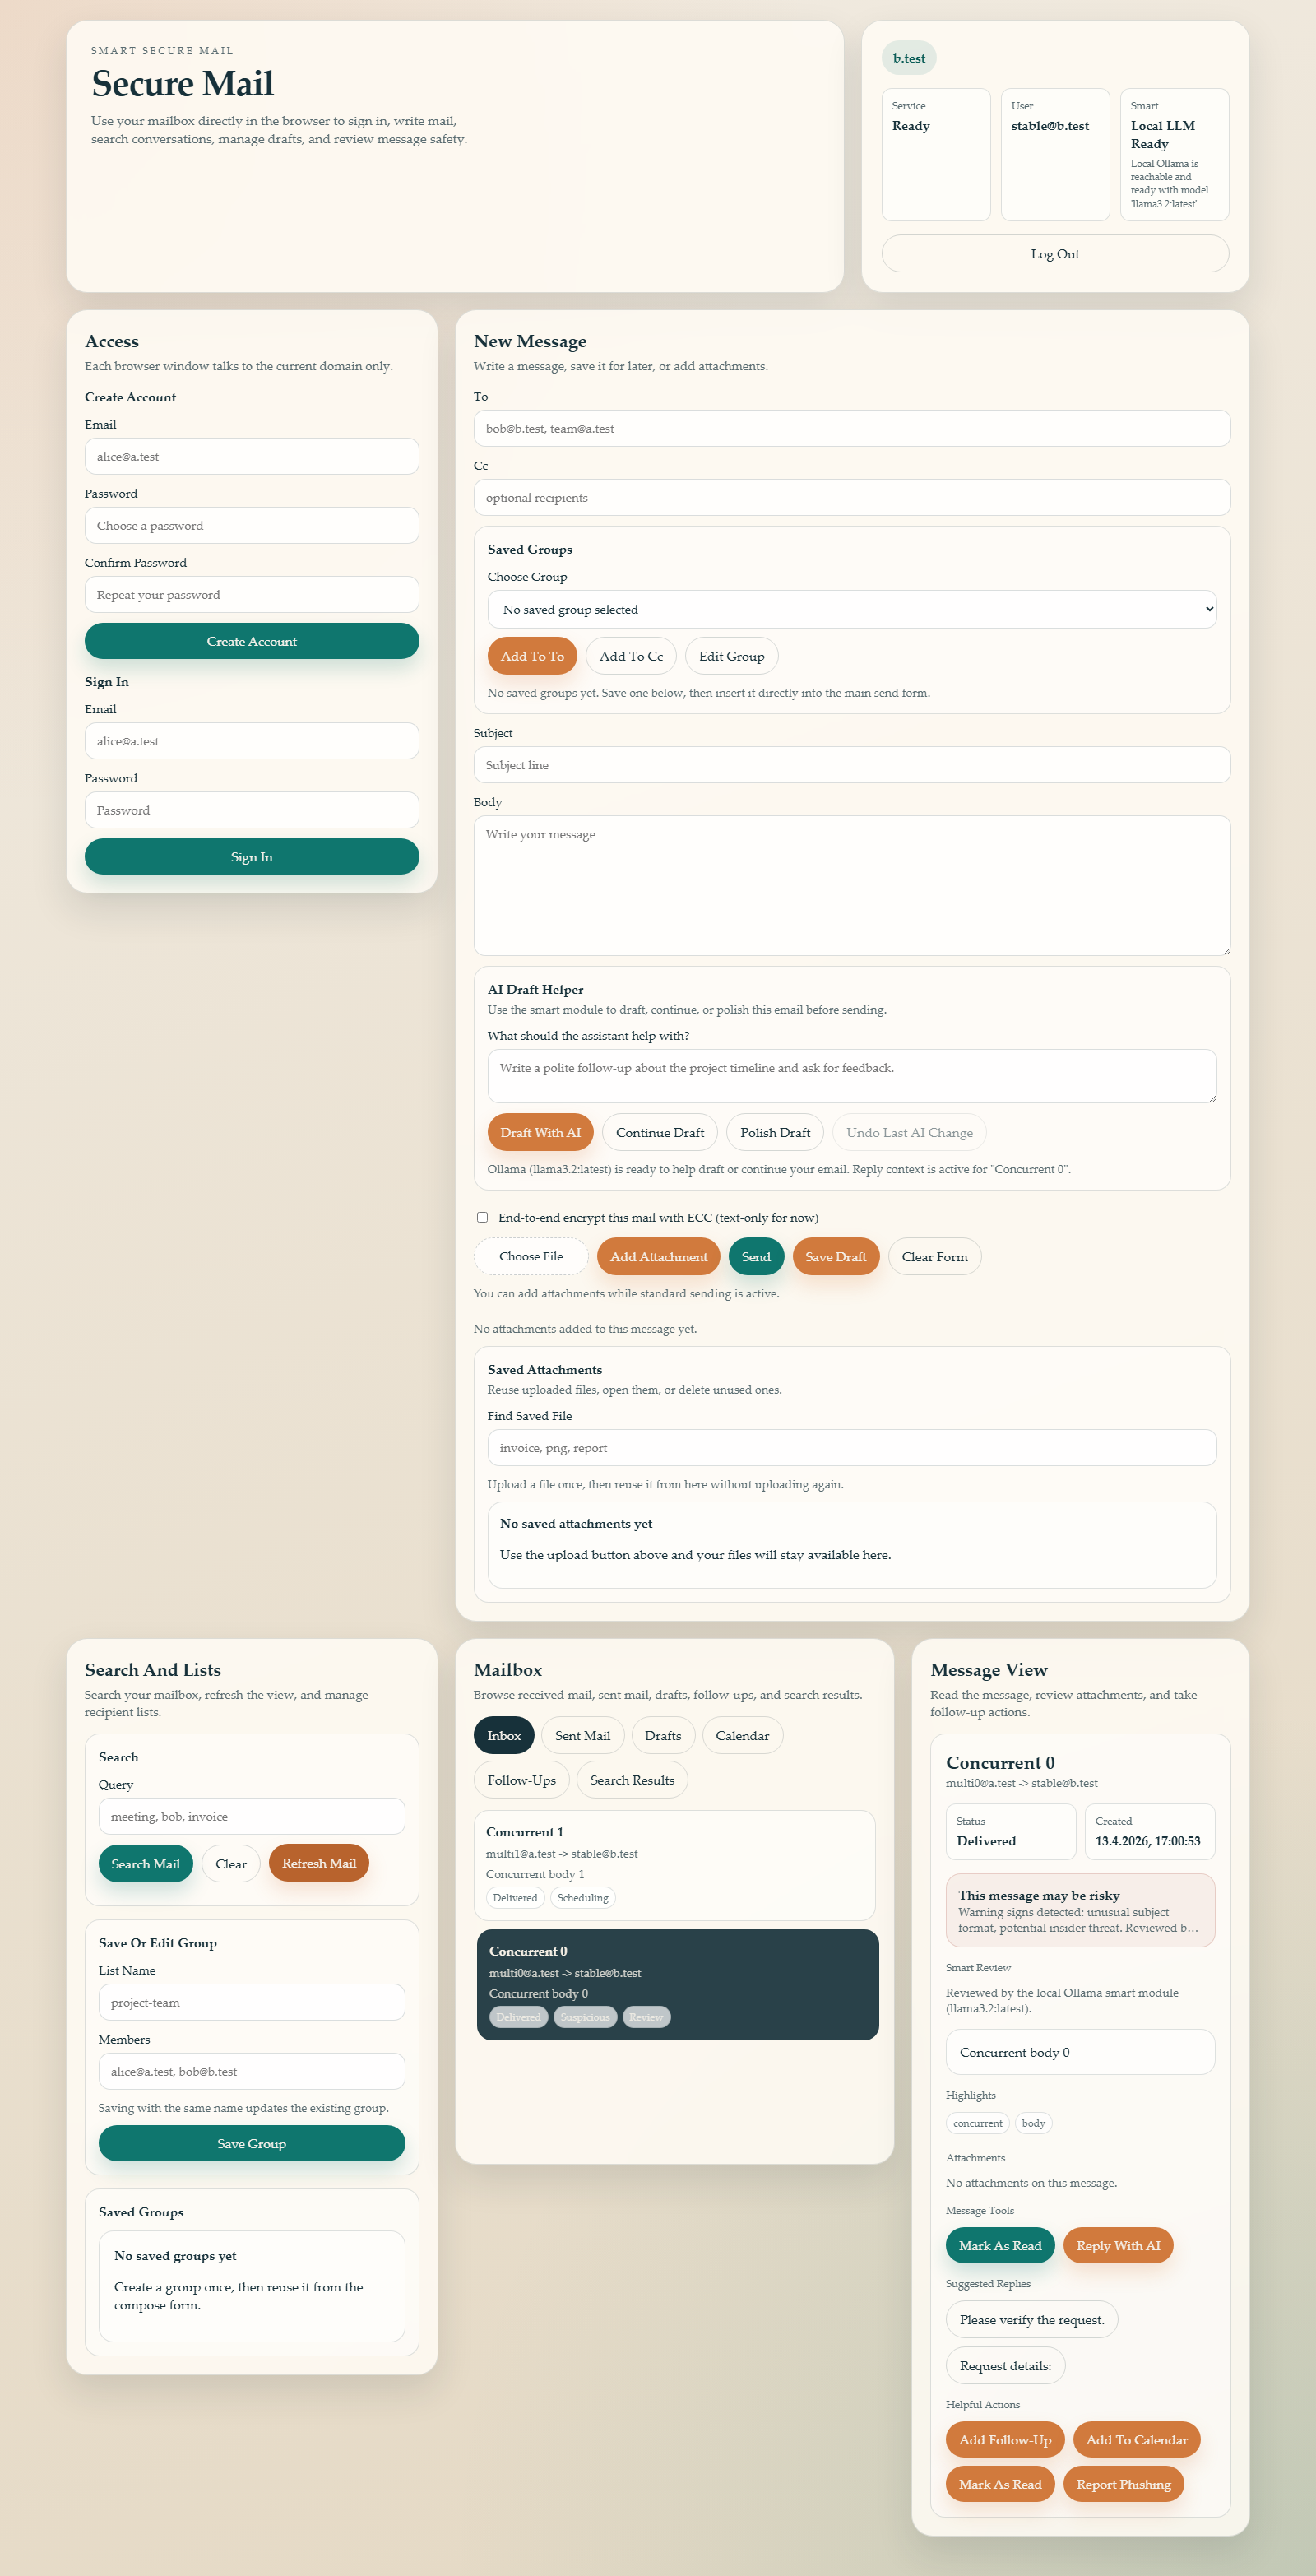
\includegraphics[width=\textwidth,height=0.50\textheight,keepaspectratio]{03_concurrency_stability_real.png}

    \vspace{0.3em}
    \scriptsize Burst delivery from many senders into one inbox.

    \column{0.49\textwidth}
    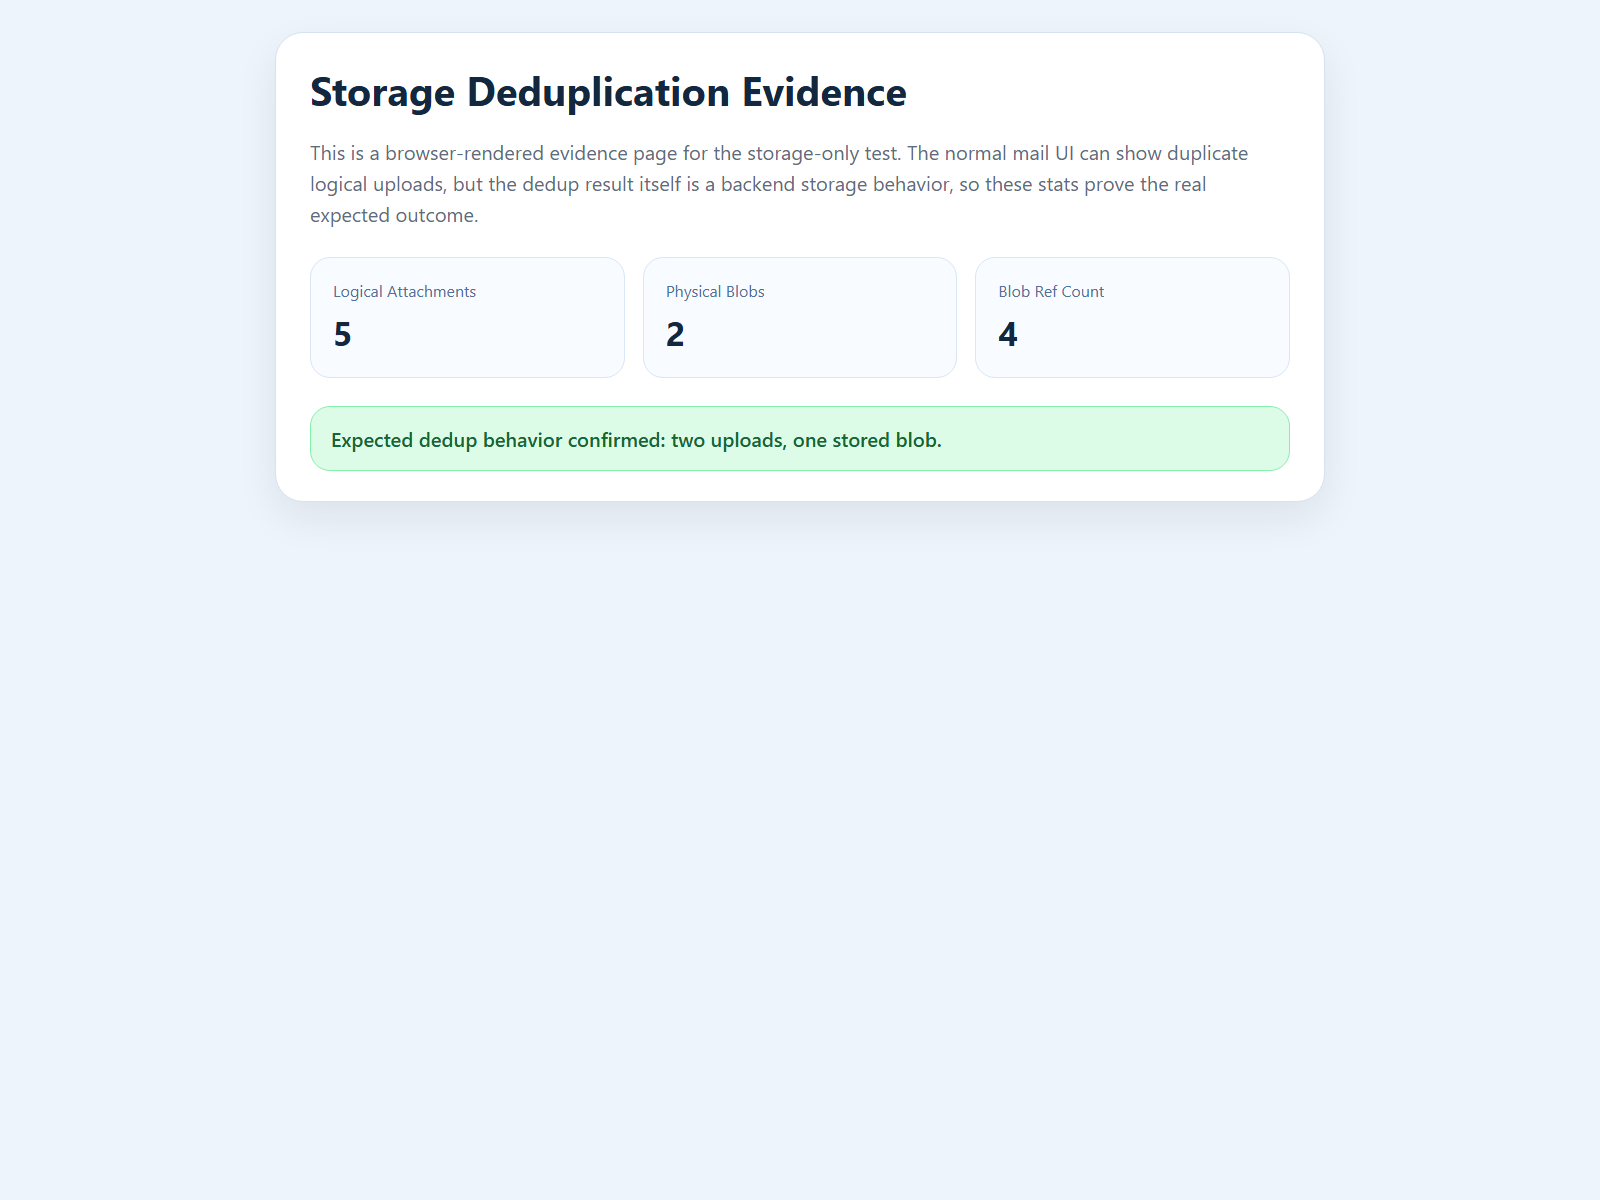
\includegraphics[width=\textwidth,height=0.50\textheight,keepaspectratio]{11_storage_dedup_backend_web.png}

    \vspace{0.3em}
    \scriptsize Browser-rendered backend evidence for deduplicated blob storage.
  \end{columns}
\end{frame}

\begin{frame}{Testing and Acceptance Coverage}
  \begin{itemize}
    \item \textbf{Functional}
    \begin{itemize}
      \item cross-domain send success
      \item inbox / sent / drafts
      \item attachments
      \item recall
      \item groups and quick actions
    \end{itemize}
    \item \textbf{Concurrency and stability}
    \begin{itemize}
      \item many users sending concurrently
      \item one recipient receiving burst traffic
    \end{itemize}
    \item \textbf{Security}
    \begin{itemize}
      \item brute-force login protection
      \item send rate limiting
      \item replay rejection
      \item tampered action rejection
      \item suspicious mail detection
    \end{itemize}
  \end{itemize}
\end{frame}

\begin{frame}{Results}
  \begin{itemize}
    \item Automated regression suite:
    \begin{itemize}
      \item \texttt{45 passed, 1 warning}
    \end{itemize}
    \item Verified scenarios include:
    \begin{itemize}
      \item queued cross-domain send
      \item CC delivery across domains
      \item login lockout
      \item rate limiting and phishing detection
      \item attachment compression, preview, and dedup behavior
      \item recall behavior
      \item web UI serving and security-lab rendering
    \end{itemize}
    \item Manual stress run completed:
    \begin{itemize}
      \item 100 different users each sent 1 mail
      \item all 100 new messages reached the target inbox
    \end{itemize}
  \end{itemize}
\end{frame}

\begin{frame}{Delivered Artifacts}
  \begin{itemize}
    \item Server and client source code
    \item Dual-domain startup scripts and configuration
    \item Protocol documentation
    \item Threat model and protection explanation
    \item Test scripts and test report
    \item Browser frontend for direct demonstration
    \item Real frontend screenshot pack and presentation PDF for mobile review
  \end{itemize}
\end{frame}

\begin{frame}{Bonus and Extension Directions}
  \begin{itemize}
    \item Malicious-script discussion is relevant because email content is attacker-controlled input.
    \item Current design reduces risk by:
    \begin{itemize}
      \item treating smart features as advisory only
      \item avoiding privileged autonomous actions
      \item escaping browser-side content
    \end{itemize}
    \item Future bonus work can include:
    \begin{itemize}
      \item end-to-end encryption design
      \item stronger audit alerting
      \item P2P mail exploration
      \item dead-letter / queue observability
    \end{itemize}
  \end{itemize}
\end{frame}

\begin{frame}{Conclusion}
  \begin{itemize}
    \item The project satisfies the assignment through a custom two-domain secure mail prototype.
    \item It combines:
    \begin{itemize}
      \item distributed-system structure
      \item practical security controls
      \item queue-based concurrency handling
      \item intelligent mailbox features
      \item reproducible testing
    \end{itemize}
    \item The final result is small enough to explain clearly, but rich enough to demonstrate engineering depth.
  \end{itemize}
\end{frame}

\end{document}
